%\section{Если из А следует B и B приятно, то A -- истина.}

В \textbf{третьей главе} построена динамическая модель экипажа на плоскости с сухим трением Амонтона -- Кулона, регуляризованным в окрестности нуля по скоростям участком линейной функции насыщения с достаточно большим угловым коэффициентом. Рассматриваются две конструкции колеса: обыкновенное омни-колесо, оси роликов которого лежат в одной плоскости, и колесо \textit{mecanum}, оси роликов которого находятся под углом к плоскости колеса. Особое внимание уделяется вопросу моделирования неудерживающей связи в контакте ролика и горизонтальной плоскости, отслеживанию точки контакта ролика и опорной плоскости, а также алгоритмической реализации процесса переключения контакта от ролика к ролику при качении омни-колеса. Динамическая модель построена в формализме объектно-ориентированного моделирования на языке Modelica. Выполнена верификация динамической модели с использованием безынерционной модели.

%\chapter{Динамика экипажа на омни-колесах с трением}
%
Наряду с постановкой задачи движения омни-колесного экипажа по абсолютно шероховатой плоскости, интерес представляет его динамика на плоскости с трением.

%с сухим трением Амонтона -- Кулона, регуляризованным в окрестности нуля по скоростям участком линейной функции насыщения с достаточно большим угловым коэффициентом, то есть достаточно сильным вязким трением.
В данной главе строится модель экипажа той же геометрии, что и выше,
но с точечным твердотельным контактом колес и роликов.
Выбрана модель сухого трения Амонтона -- Кулона. При этом, как известно~\cite{Novozhilov1991}, 
идеальный <<сухой>> случай реализовать не удается. Вместо разрывной функции 
sign от скорости относительного скольжения применяется функция линейного насыщения,
имеющая в окрестности нуля <<крутой>> линейный участок. Для таких функций известен 
результат~\cite{Novozhilov1991} о близости аппроксимирующего движения и движения, 
соответствующего <<точному>> случаю разрывной функции sign. 

%Вначале моделируется динамика ролика, совершающего свободное движение в поле сил тяжести.
%При этом предполагается, что на ролик может быть наложена неудерживающая связь --- твердотельный контакт с горизонтальной плоскостью. 
%Оказалось, что в упомянутых условиях возможно применение упрощенного и эффективного алгоритма отслеживания контакта.
%На следующем этапе реализуется модель омни-колеса, а затем -- экипажа в целом.
%Геометрия экипажа та же, что и в предыдущих главах.

Особое внимание уделяется вопросу конструирования неудерживающей связи в контакте ролика и горизонтальной плоскости,
отслеживанию точки контакта ролика и опорной плоскости,
а также алгоритмической реализации процесса 
переключения контакта от ролика к ролику при качении омни-колеса.
%Для удобства описания модели отслеживания контакта, в этой главе вводятся специальные обозначения, не связанные с принятыми в предыдущих главах.

Динамические свойства результирующей модели экипажа иллюстрируются при помощи численных экспериментов.
Проводится верификация построенной модели в сравнении с безынерционной моделью при стремлении суммарной массы роликов к нулю.

%\section{Отслеживание контакта и моделирование трения}
В разделе об \textbf{отслеживании контакта} обыкновенного омни-колеса описывается моделирование динамики ролика и строится алгоритм нахождения координат точки контакта.

%Для наглядности мы ограничиваемся рассмотрением омни-колес, 
%оснащенных четырьмя роликами. Также для простоты сами ролики имеют оси 
%вращения, лежащие в плоскости колеса (Рис.~\ref{OmniWheel}).
%
%\begin{figure}[htb]
%\centering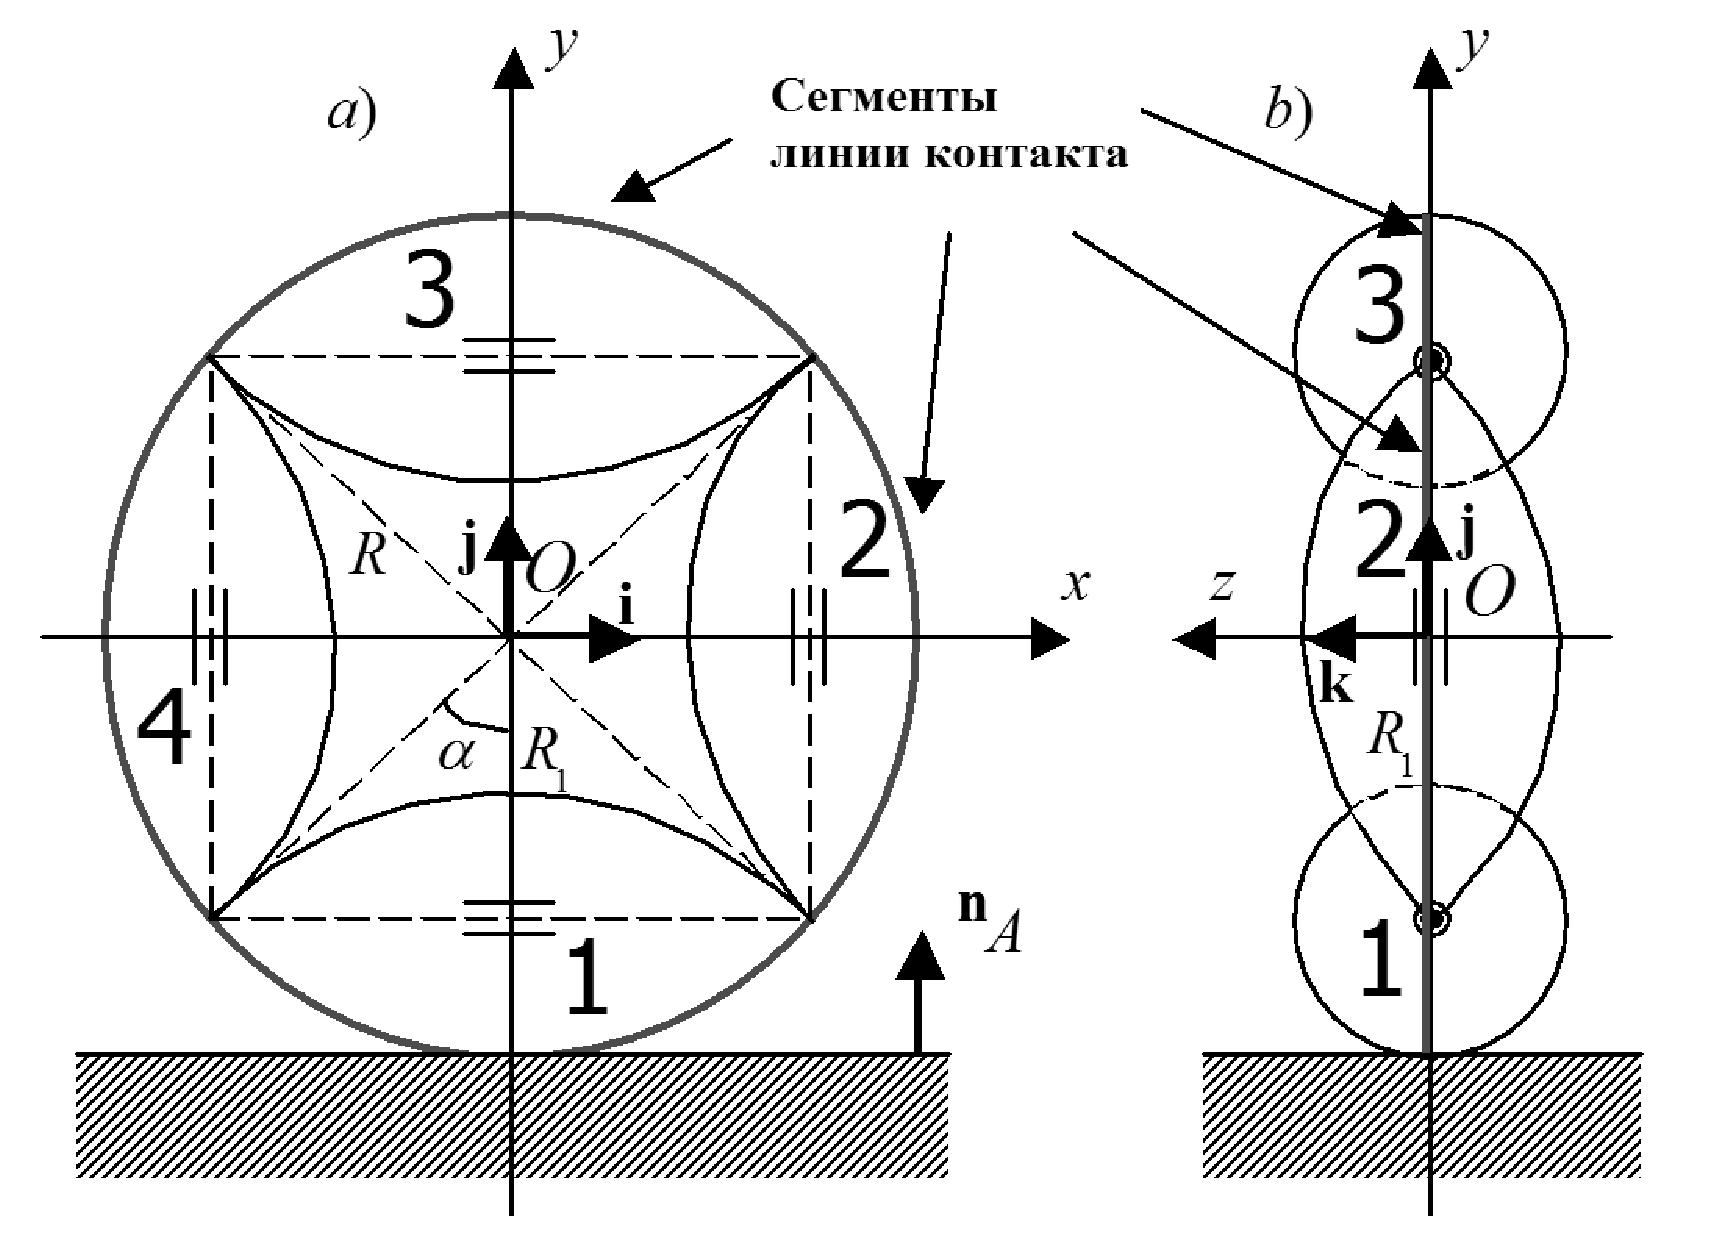
\includegraphics[width=13cm]{content/parts/3_friction/nd/OmniWheel.eps}
%\caption{Омни-колесо в вертикальном положении: a) вид сбоку; b) вид спереди.}
%\label{OmniWheel}
%\end{figure}
%
%Предполагается также, что ролики размещаются на колесе таким образом, что для 
%вертикально поставленного омни-колеса проекция линии контактирования наинизшего 
%ролика с горизонтальной плоскостью будет состоять из последовательности 
%сегментов соответствующих линий контактирования отдельных роликов. Эти сегменты 
%сопрягаются таким образом, что при переходе контакта от ролика к ролику 
%нормальная составляющая скорости точки ролика, находящейся в точке контакта, к 
%горизонтальной плоскости равна нулю. Это означает отсутствие удара по нормали к 
%плоскости. В случае коллинеарности осей роликов и плоскости колеса скачки 
%скорости скольжения по касательному направлению к горизонтальной плоскости 
%также отсутствуют, так как при переходе контакта между роликами их внешние 
%поверхности непрерывно вырождаются в точку (в идеализированной модели), что 
%означает отсутствие кинематического влияния собственного вращения роликов при 
%переходе контакта с ролика на ролик. Так что в результате переключение 
%контактов между роликами омни-колеса не приведет к нарушению регулярности 
%движения в силу причин ударного характера. Заметим еще раз, что все описанное 
%будет справедливо, если колесо все время остается в вертикальном положении.

% На следующем уровне сборки модели несколько колес соединяются с подвижной 
% платформой экипажа при помощи шарнирных связей. В нашем случае количество колес 
% может быть три или более (в зависимости от конструкции экипажа и модели 
% контактирования ролика с полом). На платформе они могут образовывать самые 
% разные конфигурации. В конкретном примере Рис.~\ref{Vehicle} имеется три 
% колеса, образующие равносторонний треугольник в горизонтальной плоскости $zx$. 
% Ось $y$ здесь предполагается вертикальной.

% \begin{figure}[htb]
% \centering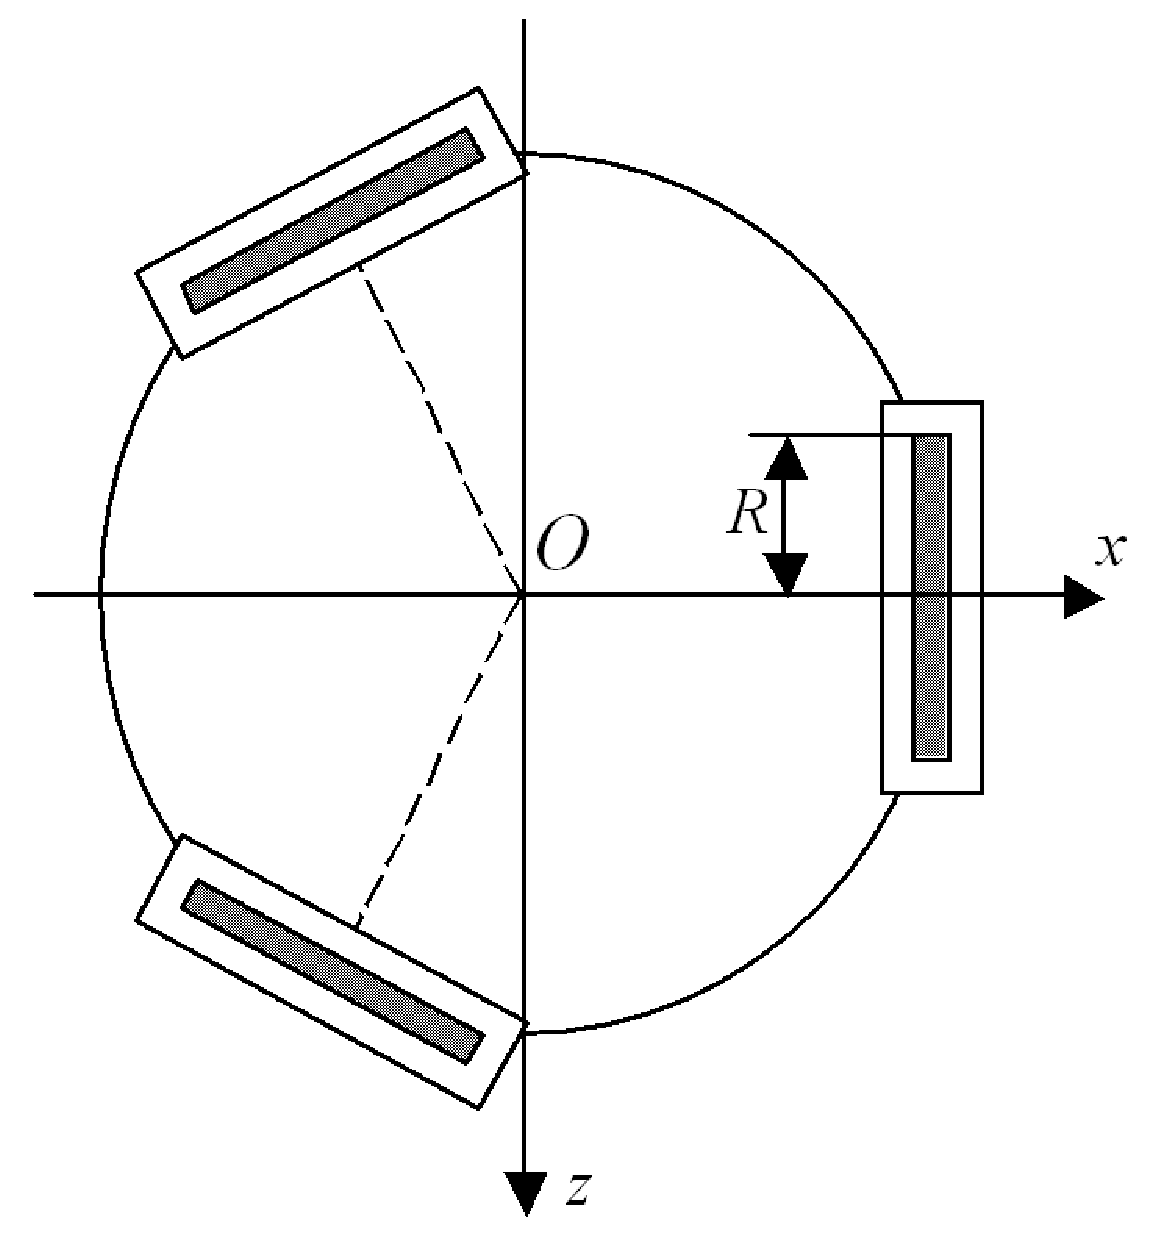
\includegraphics[width=9cm]{content/parts/3_friction/nd/Vehicle.eps}
% \caption{Трехколесный экипаж. Вид сверху.}
% \label{Vehicle}
% \end{figure}

% \section{Модель динамики отдельного ролика.\ }
%\label{sec3}
%Вначале предположим, что ролик представляет собой осесимметричное 
%веретенообразное твердое тело с внешней поверхностью, задаваемой в своих 
%собственных осях $Oxyz$ уравнением
%\begin{equation}
%x^2+\left(\sqrt{y^2+z^2}+R_1\right) ^2=R^2,
%\label{3_1}
%\end{equation}
%где $R$ --- радиус омни-колеса, $R_1=R\cos{\alpha }$ --- расстояние от центра
%ролика до центра колеса, $\alpha =\pi /n$ --- половина центрального угла, под
%которым ролик виден из центра колеса, $n$ --- количество роликов на колесе.
%
%\begin{figure}[htb]
%\centering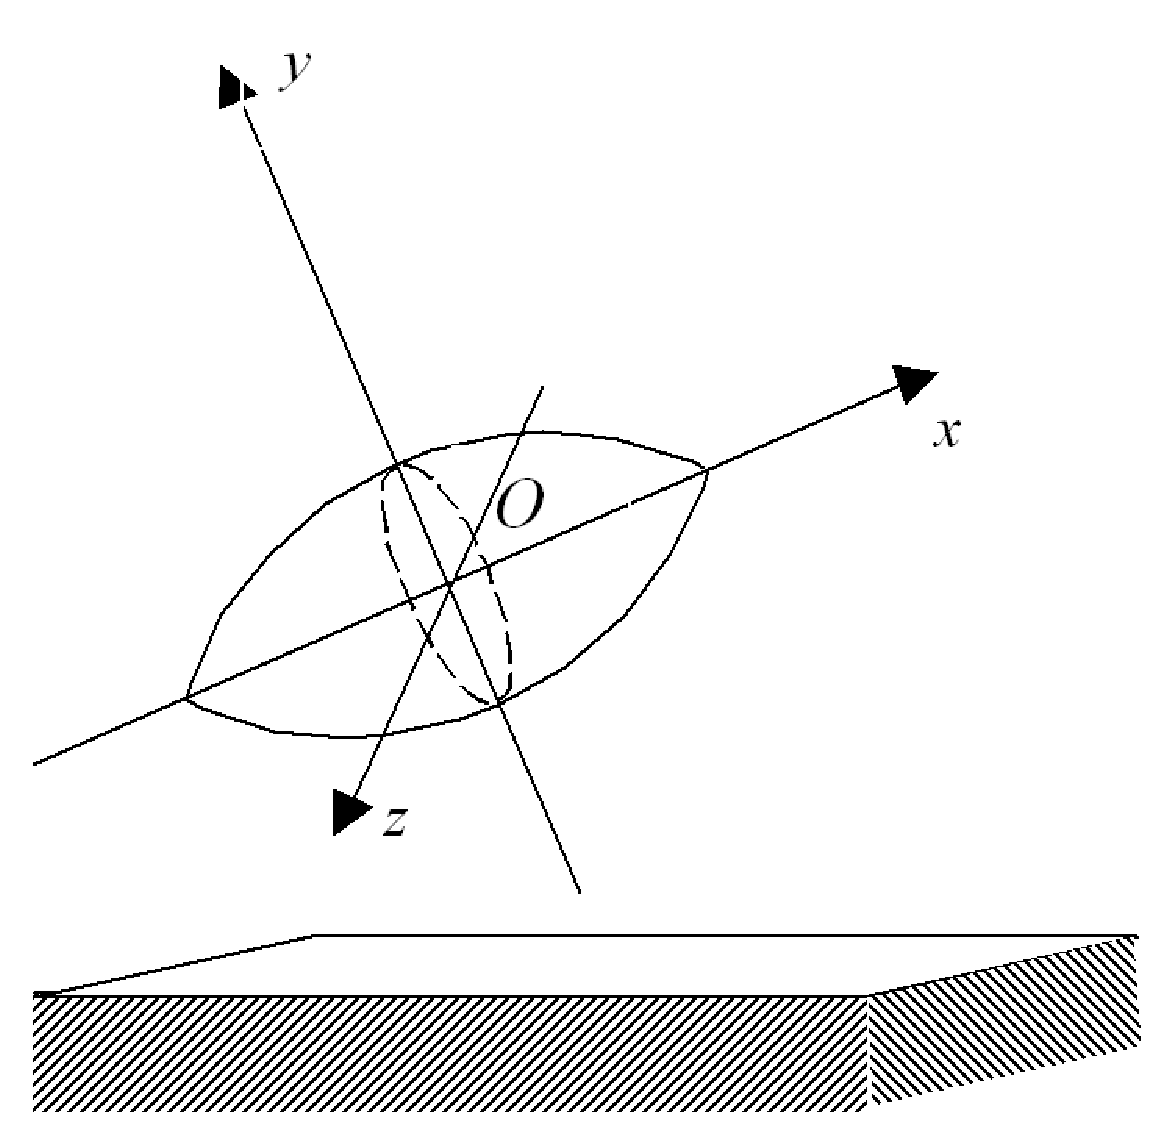
\includegraphics[width=10cm]{content/parts/3_friction/nd/Roller.eps}
%\caption{Ролик над горизонтальной плоскостью. Вид сбоку.}
%\label{Roller}
%\end{figure}

Динамика поступательно-вращательного движения реализуется так, как это описано
в~\cite{Kosenko2007}, в виде уравнений Ньютона -- Эйлера. Причем для 
моделирования вращательного движения твердого тела используется алгебра 
кватернионов~\cite{KosenkoQuaternionRus,Kosenko1998}.

Отдельную проблему представляет задача отслеживания контакта между поверхностью 
ролика и горизонтальной плоскостью. Для моделирования динамики твердого тела с
неудерживающей связью применена технология, описанная в~\cite{Kosenko2006}. В
данном случае можно было бы применить систему алгебраических или 
дифференциально-алгебраических уравнений. Однако эти уравнения вырождаются в 
точках $x=\pm R\sin\alpha $ в координатах ролика. Такое вырождение обычно 
приводит к аварийному завершению вычислительного процесса моделирования.

В нашей задаче положение спасает специфика конфигурации, обеспечивающей 
постоянство вертикального расположения омни-колес. При этом условии можно
указать явную формулу, позволяющую вычислить ближайшую к плоскости точку $P_B$
ролика (Рис.~\ref{ContactScheme}). Этой точке всегда <<противостоит>> её 
вертикальная проекция $P_A$ на плоскость (Рис.~\ref{ContactScheme}).

\begin{figure}[htb]
\centering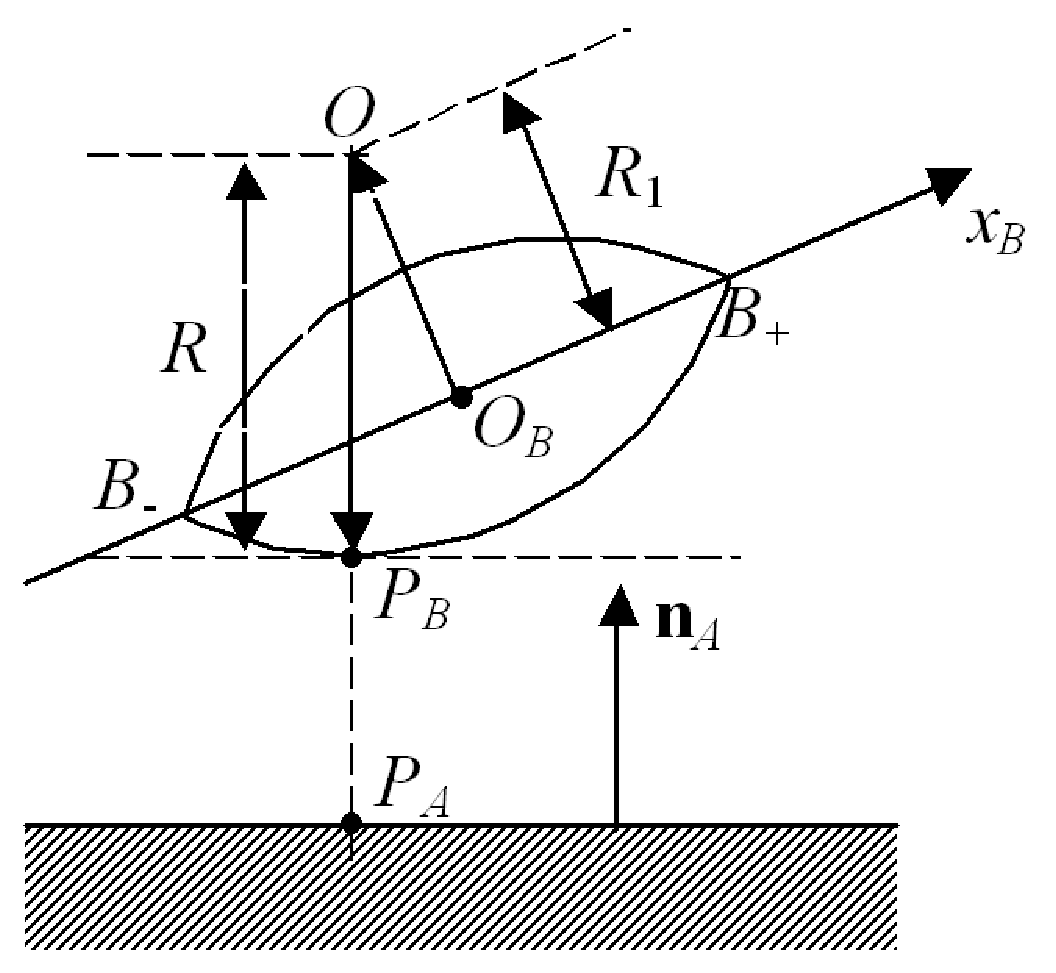
\includegraphics[width=8cm]{content/parts/3_friction/nd/RollerSection.eps}
\caption{Схема отслеживания контакта: вид сбоку отдельного ролика.}
\label{ContactScheme}
\end{figure}

%Обозначим символом ${\bf i}_B=(1,0,0)^T$ орт собственной оси ролика $O_Bx_B$.
%Этот вектор представлен в системе координат ролика $O_Bx_By_Bz_B$. Пусть $T_B$
%--- матрица поворота ролика относительно инерциальной системы координат 
%$O_Ax_Ay_Az_A$, связанной с неподвижной плоскостью. Пусть также ${\bf r}_B$ ---
%радиус-вектор геометрического центра ролика в текущий момент времени и 
%${\bf n}_A=(0,1,0)^T$ --- орт нормали (восходящей вертикали) к плоскости. 
%Плоскость условно обозначается нами телом с индексом $A$, ролик --- $B$. Пусть
%${\bf d}$ --- горизонтальный орт, вычисляемый по формуле
%$$
%{\bf d}=\dfrac{T_B{\bf i}_B\times {\bf n}_A}
%              {\left| T_B{\bf i}_B\times {\bf n}_A\right|}.
%$$
%Тогда, очевидно, отрезок $\overrightarrow{O_BO}$, расположенный в вертикальной
%плоскости, будет иметь длину $R_1$ и задаваться формулой
%$$
%\overrightarrow{O_BO}=R_1{\bf d}\times T_B{\bf i}_B.
%$$
%Здесь $O$ --- центр кривизны окружности вертикального сечения ролика 
%(Рис.~\ref{ContactScheme}).
Самая нижняя точка $P_B$ внешней 
поверхности ролика будет задаваться по формуле
\begin{equation}
{\bf r}_{P_B}={\bf r}_B+R_1{\bf d}\times T_B{\bf i}_B-R{\bf n}_A,
\label{3_2_0}
\end{equation}
поскольку точка $P_B$ лежит на упоминавшейся выше окружности на общей вертикали 
с точкой $O$.
Вместе с тем необходимо потребовать нахождения радиус-вектора центра ролика
относительно центра колеса на угловом расстоянии не более половины углового размера ролика от вертикали,
а также, а также нахождения точки контакта ниже центра колеса.
%Для вычисления положения точки $P_A$ нужно вторую координату 
%вектора ${\bf r}_{P_B}$ положить равной нулю
%\begin{equation}
%{\bf r}_{P_A}=\left( x_{P_B},0,z_{P_B}\right) ^T.
%\label{3_2_1}
%\end{equation}

%Вся описанная выше вычислительная процедура будет справедлива только, если 
%вектор $T_B{\bf i}_B$ имеет направление, ограниченное по вертикали углами
%$\pm\alpha $. Если соответствующий угол превышает значение $\alpha $, то 
%следует положить $P_B=B_{-}$, где $B_{-}$ --- левая концевая точка ролика. Если
%же этот угол меньше величины $-\alpha $, нужно положить $P_B=B_{+}$, где 
%$B_{+}$ --- правая концевая точка ролика.

%В конечном итоге условие контактирования ролика и плоскости можно записать в 
%виде
%\begin{equation}
%\left| T_B{\bf i}_B\cdot {\bf n}_A\right|\le\sin\alpha .
%\label{3_2}
%\end{equation}
%Это условие, однако, позволяет из всего множества роликов колеса выделить 
%нижний (контактирующий) и верхний. Чтобы отбросить случай последнего ролика
%можно к последнему условию присоединить также требование 
%\begin{equation}
%y_B<R,
%\label{3_3}
%\end{equation}
%где $y_B$ --- высота центра ролика относительно инерциальной системы координат.

%Одновременное выполнение описанных условий означает наличие
%контакта. В противном случае, при отсутствии контакта, нормальная реакция 
%отсутствует (закон Синьорини). С другой стороны, реализация контакта 
%геометрически означает выполнение скалярного условия 

Одновременное выполнение описанных условий означает наличие
контакта и означает выполнение скалярного условия 
\begin{equation}
y_{P_B}=0,
\label{3_4}
\end{equation}
а в противном случае имеет место скалярное условие
$$
F_n=0,
$$
где $F_n$ --- нормальная составляющая реакции, приложенной в точке $P_B$ (закон Синьорини).

% \begin{figure}[htb]
% \centerline{
% 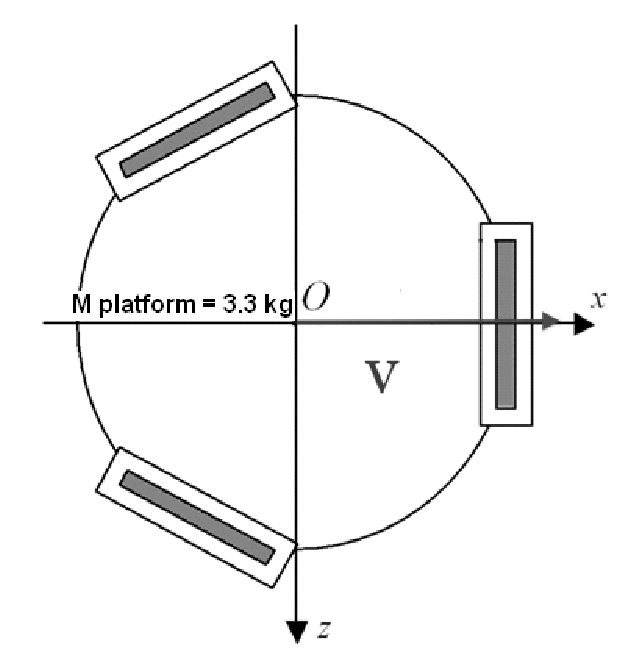
\includegraphics[width=7cm]{content/parts/3_friction/nd/Translat.eps}
% 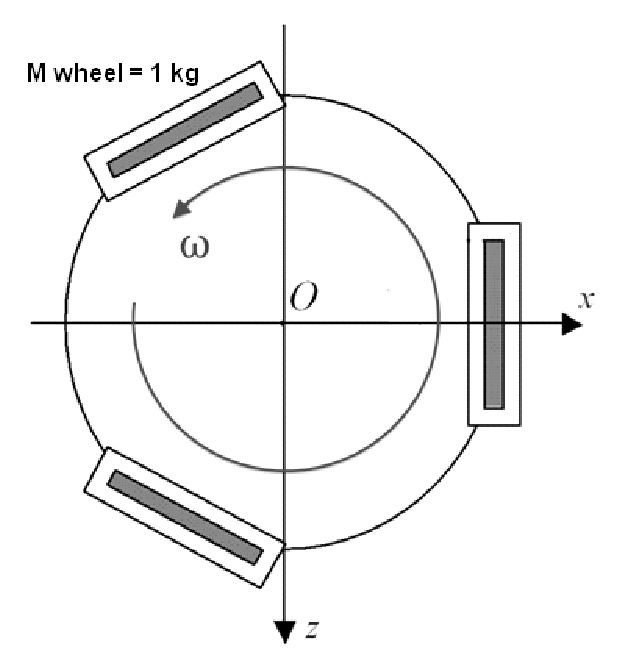
\includegraphics[width=7cm]{content/parts/3_friction/nd/Rotat.eps}
% }
% \caption{Типы движения при верификации модели.}
% \label{TypesOfMotion}
% \end{figure}

Отмечается, что использование условия (\ref{3_4}) во время численного решения
непосредственно в указанной форме стабильно приводит к аварийному завершению процесса симуляции.
Аналогично для первой производной этой формы по времени.
Для корректной работы объекта контактирования
(реализованного в данном случае на языке Modelica~\cite{Fritzson})
требуется задать это условие в форме его второй производной $\dot{v}_n=0$.

%Вычислительная практика показала, что уравнения контакта в форме (\ref{3_4})
%стабильно приводит к аварийному завершению процесса симуляции динамической 
%модели ролика. Аналогичный результат получается, если в качестве уравнения 
%контактирования использовать уравнение вида 
%$$
%v_n=0,
%$$
%где $v_n$ -- нормальная составляющая скорости точки контактирования, лежащей
%на теле $B$, относительно тела $A$ (горизонтальной плоскости). И только 
%уравнение вида
%$$
%\dot{v}_n=0
%$$
%приводит к требуемому результату -- корректной работе объекта контактирования
%(реализованного в данном случае на языке Modelica~\cite{Fritzson}) в процессе 
%симуляции модели.
%Вся реализация процесса контактирования 
%выполнена в предположении точечного <<твердого>> контакта твердых тел без 
%какой-либо податливости.
%
%Колеса, собранные в экипаж, с неизбежностью будут сохранять вертикальное 
%положение. Поэтому упрощенный алгоритм отслеживания контакта, описанный выше,
%всегда будет работать правильно.

%\section{Отслеживание контакта в случае \textit{mecanum} колеса}
В разделе об \textbf{отслеживании контакта в случае \textit{mecanum} колеса} строится два алгоритма для нахождения координат точки контакта: явный и неявный, сравниваются решения, полученные в соответствии с каждым, и вычислительная эффективность алгоритмов.

%Обозначим угол наклона оси ролика к плоскости колеса $\psi$. В предыдущей конфигурации этот угол равен нулю. Расширим алгоритм отслеживания контакта, описанный выше для случая $\psi = 0$ на конфигурацию \textit{mecanum}, $\psi > 0$. В этом случае, в первую очередь, отметим отличия в геометрической форме роликов. Каждый ролик -- это твердое тело, ограниченное поверхностью вращения некоторой кривой вокруг его оси. В случае $\psi = 0$ эта кривая -- дуга окружности, но при $\psi > 0$, для того, чтобы проекция внежней границы колеса на его плоскость оставалась окружностью, форма роликов должна быть более сложной \cite{Gfrerrer2008}.
%
%\subsection{Неявный алгоритм отслеживания контакта}
\textbf{Неявный алгоритм отслеживания контакта} основан на наблюдении, что точка контакта находится всегда в пересечении вертикальной плоскости, содержащей ось колеса, и горизонтальной опорной плоскости. Координаты проекции центра колеса на опорную плоскость могут быть вычислены явно, и остается получить лишь расстояние $\mu$ от этой проекции до точки контакта вдоль отрезка линии пересечения плоскостей, соединяющего их, см. рис УКАЗАТЬ.

Величина $\mu$ может быть выражена из равенства
$$
{\bf r}_{P_B}={\bf r}_{O_B}+R_1\vecrho -R{\bf j}_1+\mu {\bf k}_1,
$$
после умножения его скалярно на ${\bf k}_2$:
$$
\mu =\left[R{\bf j}_1\cdot{\bf k}_2-R_1{\vecrho }\cdot {\bf k}_2\right] /
{\bf k}_1\cdot{\bf k}_2,
$$
где компоненты вектора $\vecrho$ находятся с помощью кинематических соотношений
$$
\vecrho\cdot {\bf i}_2=0,\quad\vecrho\cdot {\bf k}_1=0,
$$
а точнее, учитывая специфику численного решения, интегрированием их дифференциальных версий:
$$
\dfrac{d}{dt}\vecrho\cdot {\bf i}_2+\vecrho\cdot\dfrac{d}{dt}{\bf i}_2=0,\quad
\dfrac{d}{dt}\vecrho\cdot {\bf k}_1+\vecrho\cdot\dfrac{d}{dt}{\bf k}_1=0,
$$
а компоненты векторов ${\bf i}_{(\cdot)},{\bf j}_{(\cdot)}$ известны из знания ориентации тел в пространстве.

%Здесь, как и всюду, будем предполагать, что плоскость колеса вертикальна во все время движения.
%
%Введем систему отсчета $O_A{\bf i}{\bf j}{\bf k}$, жестко связанную с колесом, с началом в его центре $O_A$. Вектор ${\bf k}$ направлен вдоль оси колеса, ${\bf i}$ и ${\bf j}$ лежат в его плоскости.
%
%Введем также две вспомогательные системы отсчета $O_A{\bf i}_1{\bf j}_1{\bf k}_1$ и $O_B{\bf i}_2{\bf j}_2{\bf k}_2$, где $O_B$ -- центр ролика.
%
%Вектор ${\bf i}_2$ направим вдоль оси симметрии ролика, см. фиг.~\ref{ContactScheme}.
%Вектор ${\bf j}_2$ ортогонален ${\bf i}_2$ и лежит в вертикальной плоскости.
%Третий вектор ${\bf k}_2$ определяется естественным образом как
%$$
%{\bf k}_2={\bf i}_2\times {\bf j}_2.
%$$
% \begin{figure}[hb]
% \centerline{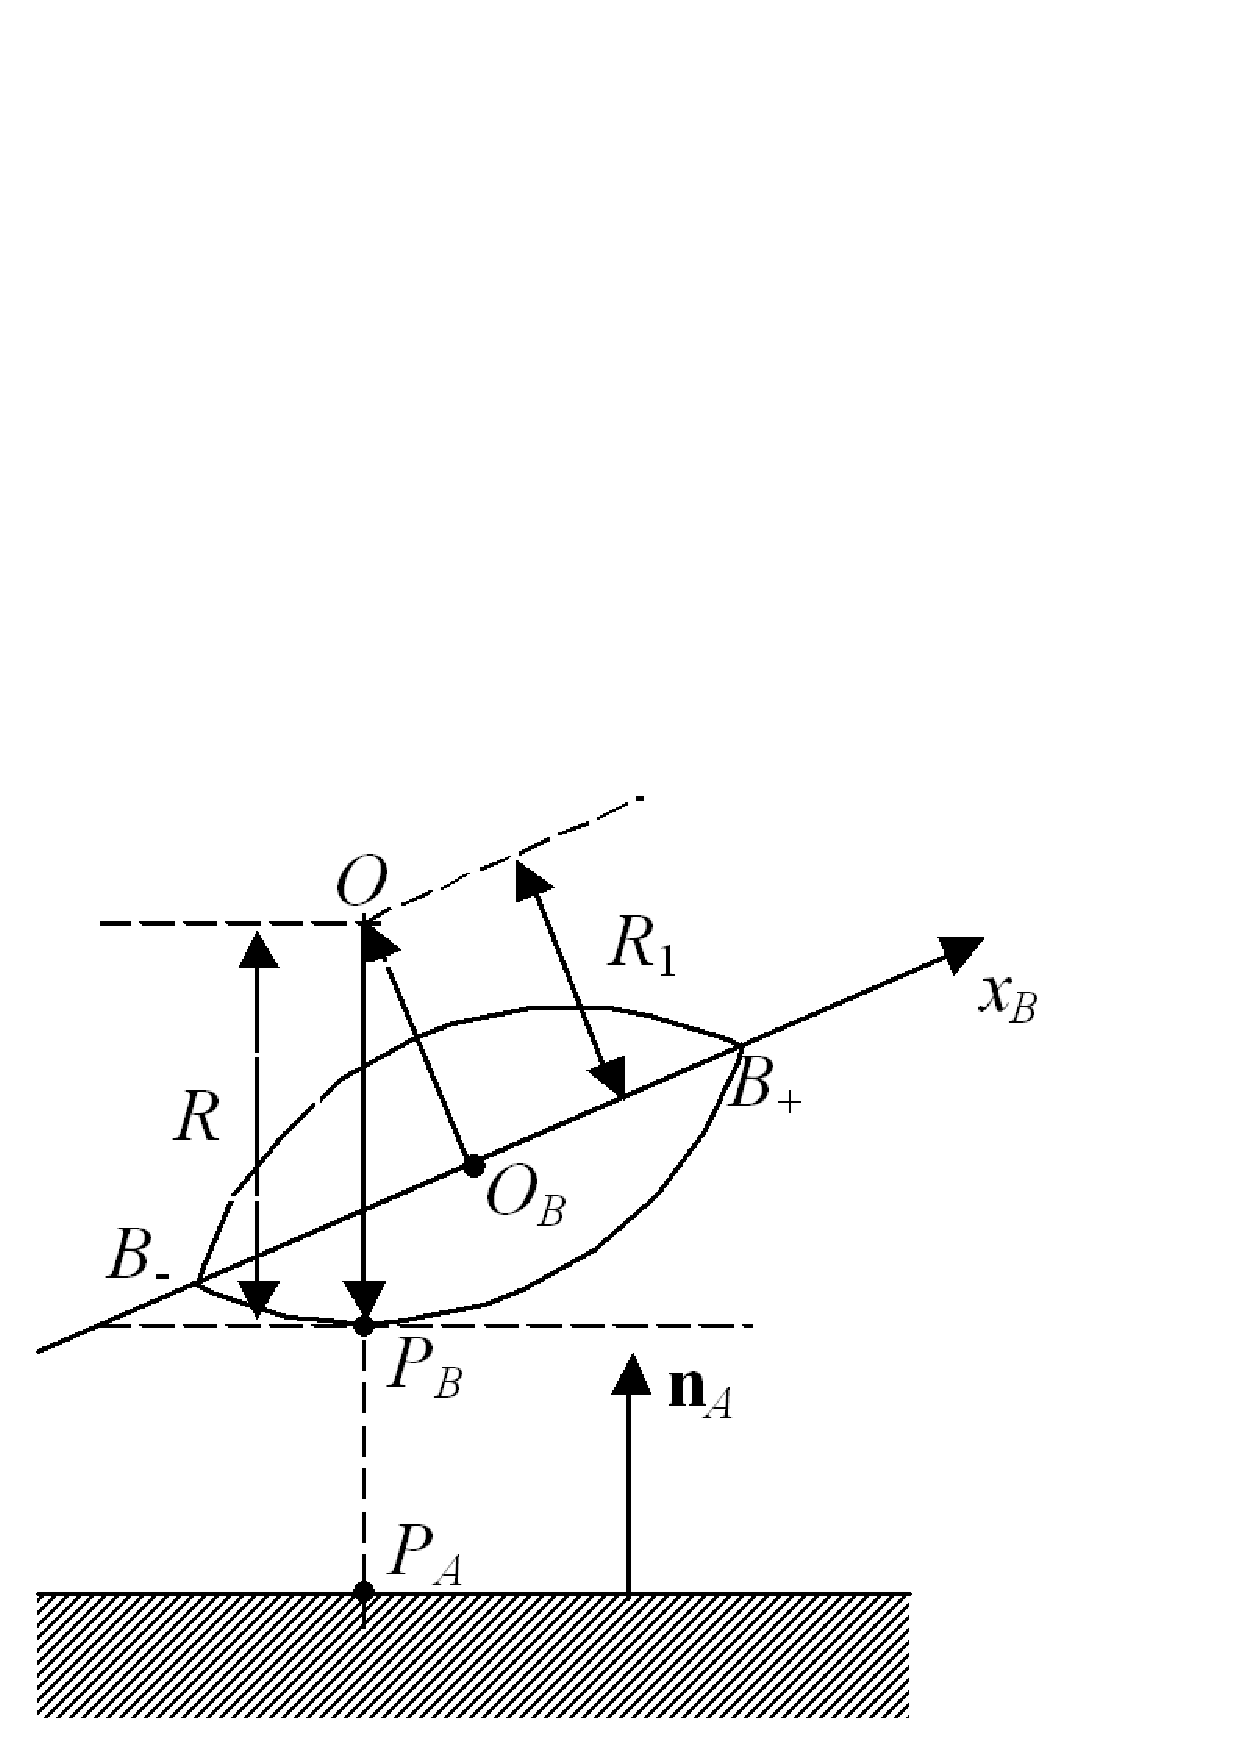
\includegraphics[bb= 0cm 0cm 20cm 17cm,scale=0.30]{RollerSection.png}}
% \caption{Contact tracking scheme.}
% \label{ContactScheme}
% \end{figure}
%
%Во время счета компоненты всех векторов задаются относительно неподвижной системы отсчета, а положения и ориентации всех тел системы в момент времени $t\in [t_0,t_1]$ считаются известными.
%
%Таким образом, для системы $O_B{\bf i}_2{\bf j}_2{\bf k}_2$, имеем:
%$$
%{\bf i}_2=T_B\cdot (1,0,0)^T,\quad\vecrho =
%\left( {\bf r}_{O_A}-{\bf r}_{O_B}\right) /
%\left| {\bf r}_{O_A}-{\bf r}_{O_B}\right| ,
%$$
%где $T_B$ -- матрица ориентации ролика, а единичный вектор $\vecrho$ направлен вдоль луча, выпущенного из центра колеса $O_A$ в сторону центра ролика $O_B$.
%
%Вектор ${\bf i}_1$ лежит на пересечении плоскости колеса и горизонтальной плоскости.
%${\bf k}_1 = {\bf k}$ ортогонален плоскости колеса и совпадает с одним из векторов базиса, связанного с колесом, и всегда горизонтален.
%Тогда имеем ${\bf j}_1(t)=(0,1,0)^T$ и ${\bf i}_1(t)={\bf j}_1(t)\times {\bf k}_1(t)$.
%
%Теперь рассмотрим соотношения, позволяющие вычислить компоненты базисных векторов векторов системы отсчета $O_B{\bf i}_2{\bf j}_2{\bf k}_2$.
%
%Отметим, что вектор ${\bf i}_2$, направленный вдоль оси ролика, по определению не может принять вертикальное положение, если ролик находится в контакте с опорной плоскостью.
%Более того, в случае \textit{mecanum} ролик повернут на постоянный угол $\psi > 0$ относительно оси $O_AO_B$, и потому во все время движения верно соотношение ${\bf i}_2\ne (0,1,0)^T$.
%Таким образом, вектор ${\bf c}={\bf i}_2\times (0,1,0)^T$ также отличен от нуля.
%Положим ${\bf k}_2={\bf c}/|{\bf c}|$. Теперь можно определить ${\bf j}_2$ как
%${\bf j}_2={\bf k}_2\times {\bf i}_2$.

%Для определения компонент вектора $\vecrho$ воспользуемся кинематическими соотношениями, условиями ортогональности векторов, следующими из определений введенных систем отсчета:
%$$
%\vecrho\cdot {\bf i}_2=0,\quad\vecrho\cdot {\bf k}_1=0.
%$$
%и их дифференциальными вариантами:
%$$
%\dfrac{d}{dt}\vecrho\cdot {\bf i}_2+\vecrho\cdot\dfrac{d}{dt}{\bf i}_2=0,\quad
%\dfrac{d}{dt}\vecrho\cdot {\bf k}_1+\vecrho\cdot\dfrac{d}{dt}{\bf k}_1=0.
%$$
%
%Величина $c_{\beta }=\cos\beta ={\bf i}_2\cdot (0,1,0)^T$ косинуса угла $\beta $ наклона оси ролика к вертикали $(0,1,0)^T$ также играет важную роль в алгоритме отслеживания контакта.
%
%Если текущее значение переменной величины $c_{\beta }$ меньше некоторого уровня $c_{\beta\max }$, и если одновременно расстояние от центра ролика $O_B$ до опорной плоскости меньше радиуса колеса $R$, то ролик находится в контакте с опорной плоскостью. В противном случае контакт отсутствует.

% Remark here that usually to arrange the unilateral constraint in the multibody
% system dynamics model the developer has to implement anything like hybrid 
% automata construct. In our omni wheel model on the contrary this is not the 
% case. It turned out sufficient to implement ``simple'' ``{\tt if}'' construct 
% to switch states ``contact'' and ``no contact'' for each individual roller, and
% simultaneously to advance forward ``contact'' state from one roller to its 
% neighbour. The whole picture looks like from time to time neighbouring rollers
% mutually exchange by their states.

%На фиг.~\ref{ContactScheme} также легко видеть, что координаты точки $P_B$ контакта ролика и плоскости даются выражением
%$$
%{\bf r}_{P_B}={\bf r}_{O_B}+R_1\vecrho -R{\bf j}_1+\mu {\bf k}_1,
%$$
%где число $\mu$ требуется вычислить. Здесь величина $R_1$ равна расстоянию между точками $O_A$ и $O_B$.
%Чтобы получить число $\mu$, умножим последнее уравнение скалярно на ${\bf k}_2$. Отсюда
%$$
%\mu =\left[R{\bf j}_1\cdot{\bf k}_2-R_1{\vecrho }\cdot {\bf k}_2\right] /
%{\bf k}_1\cdot{\bf k}_2,
%$$
%поскольку ${\bf r}_{P_B}-{\bf r}_{O_B}$ лежит в вертикальном сечении осесимметричной поверхности ролика, и вектор ${\bf k}_2$ по построению ортогонален этому сечению. В результате радиус-вектор ${\bf r}_{P_B}$ точки контакта $P_B$ определяется однозначно.

%\section{Явный алгоритм отслеживания контакта}
Далее описывается \textbf{явный алгоритм отслеживания контакта}. Еще одним способом вычисления компонент радиус-вектора ${\bf r}_{P_B}$ точки контакта point $P_B$ или, точнее, точки ролика, ближайшей к опорной плоскости, является применение следующего набора равенств.
Лучше всего этот способ иллюстрирует геометрическая схема на фиг.~\ref{fig:figure3}. Во-первых, имеем
$$
{\bf r}_{P_B}={\bf r}_{O_B}+\overrightarrow{CD}+\overrightarrow{DG},\quad
\overrightarrow{CD}=-m{\bf i}_2,\quad\overrightarrow{DG}=-h{\bf j}_1,
$$
где $m=R_1\sin q/\cos q/\cos\psi $, $h=R-R_1/\cos q$. Здесь $q$ -- текущее значение угла отклонения вектора ${\bf r}_{O_A}-{\bf r}_{O_B}$ от 
направления вектора $\overrightarrow{DO}$. Таким образом,
$$
\cos q=\vecrho\cdot{\bf n}_A,\quad\sin q=
\left({\bf n}_A\times\vecrho\right)\cdot {\bf k}_1.
$$
\begin{figure*}[ht]
\centerline{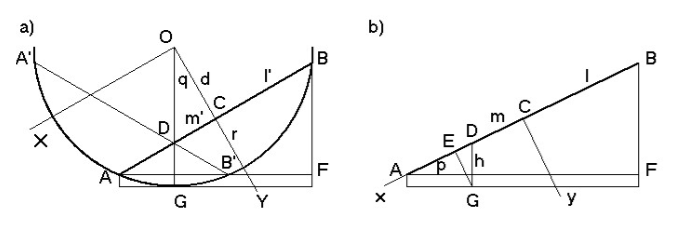
\includegraphics[scale=0.7]{content/parts/3_friction/mo2015/stepanov.png}}
\caption{Явная схема отслеживания контакта}
\label{fig:figure3}
\end{figure*}

%Поясним фиг.~\ref{fig:figure3} более детально.
%В части (а) приведена проекция колеса на его плоскость и соответственно, проекция ролика, находящегося в общем положении так, что его ось находится под углом к плоскости проекции.
%Далее, $G$ -- точка контакта между роликом и опорной горизонтальной плоскостью в настоящий момент, $m'$ -- отрезок $DC$ проекции оси ролика на плоскость колеса. Лекго видеть, что длина этой проекции равна $m'=m\cos\psi$, поскольку ось ролика $AB$ повернута вокруг прямой $OC$ на угол $\psi$, см. вертикальное сечение, содержащее ось ролика в части (b).
%Таким образом, чтобу получить точку контакта $P_B$ ($G$ на рис.), нужно пройти два отрезка прямых от центра ролика $O_B$ ($C$ на рис.): (a)~отрезок $CD$ оси ролика длины $m$; 
%(b)~отрезок $DG$ вертикали длины $h$.
%Как было отмечено выше, все величины требуется явно выразить через известные координаты.
%
%Чтобы исключить <<перекрытие>> роликов, т.е. ситуацию, при которой два ролика могут находиться в контакте одновременно, более чем при одном (граничном) значении угла поворота колеса, необходимо ограничить длины роликов величиной (см. фиг.~\ref{fig:figure3})
%$$
%L=2R\sin\alpha / \cos\psi,
%$$
%и при этом их концы оказываются усечены. Подробно форма кривой, образующей поверхность роликов, описана в \cite{Gfrerrer2008}.
%При такой конструкции переход колеса с одного ролика на другой происходит мгновенно.

Описанные алгоритмы отслеживания контакта дают практически одинаковые результаты, относительные различия между которыми имеют порядок $10^{-8}$. Предсказуемо, явный алгоритм быстрее приблизительно в $1.5$ раза.

При переходе колеса конструкции \textit{mecanum} с одного ролика на другой его след на плоскости терпит разрыв, поскольку точка контакта мгновенно переходит на противоположный <<борт>> колеса. Отметим, что это обстоятельство, тем не менее, не препятствует эффективному численному решению.

%В процессе отладки модели рассматривались автономные движения отдельного омни-колеса.
%
%Заметим, что перед началом процесса редукции индекса системы 
%диф\-фе\-рен\-ци\-аль\-но-алгебраических уравнений полной модели экипажа, реализованного
%в программном обеспечении лаборатории ди\-на\-ми\-чес\-ко\-го моделирования 
%Dymola~\cite{Dymola}, эта модель составляется из: а) твердого тела платформы
%омни--экипажа; б) трех твердых тел -- моделей омни--колес; в) двенадцати 
%твердых тел роликов, размещенных на колесах. В соответствии, например, 
%с~\cite{Kosenko2007} для каждого объекта, моделирующего твердое тело, 
%реализуются шесть обыкновенных дифференциальных уравнений (ОДУ) Ньютона для
%движения центра масс тела плюс семь ОДУ Эйлера для вращательного движения тела
%вокруг центра масс. В последнем случае имеется четыре кинематических уравнения
%Эйлера для кватерниона ориентации тела плюс три динамических уравнения Эйлера
%для вектора угловой скорости твердого тела. В результате полная модель экипажа
%задается системой ОДУ порядка $16\cdot 13=208$. Кроме этого, объекты 
%механических связей могут генерировать дополнительные дифференциальные 
%уравнения.

В ходе численных испытаний проверено, что абсолютная величина ошибки соблюдения неудерживающей связи 
остается пренебрежимо малой -- около $10^{-7}$ от единицы длины.

%
%\begin{figure}[htb]
%\centerline{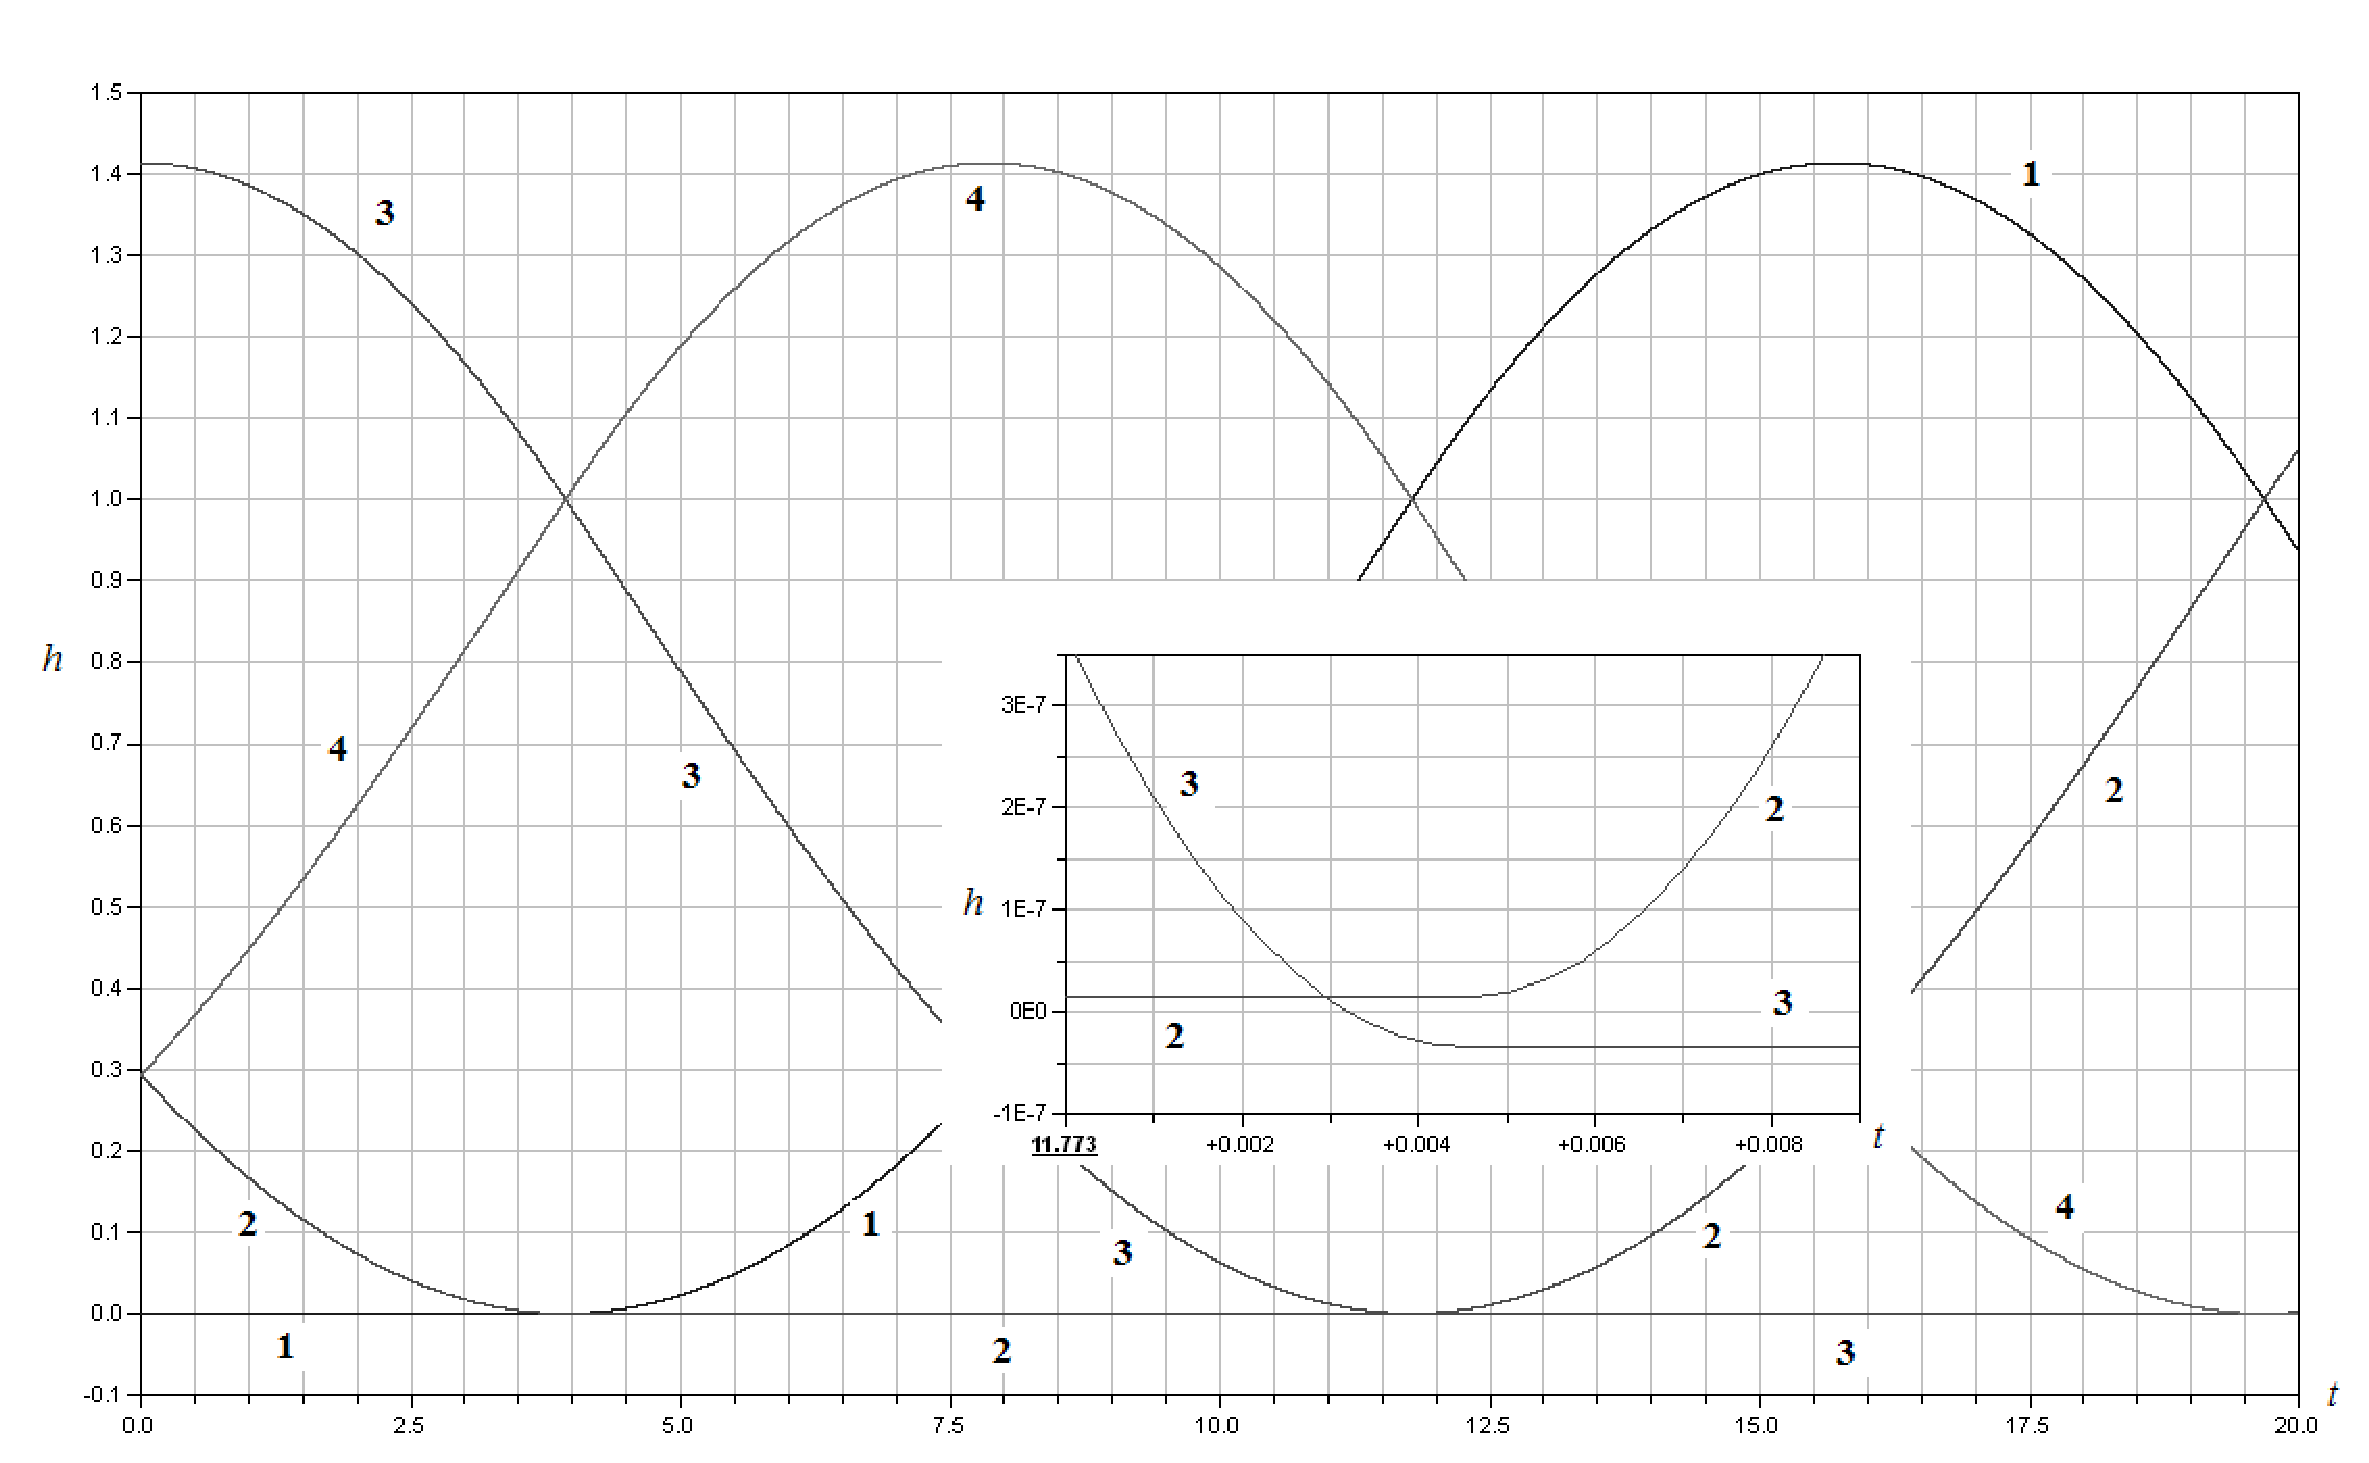
\includegraphics[width=15cm]{content/parts/3_friction/nd/Figure11.eps}}
%\caption{Процесс замещения роликов в контакте.}
%\label{fig1}
%\end{figure}
%
%Эволюция процесса контактирования для отдельного катящегося омни-колеса 
%показана на Рис.~\ref{fig1}, где представлены зависимости функций расстояний 
%$h$ (фактически -- высот) между горизонтальной плоскостью (полом) и роликами 
%одного и того же колеса, находящимися в разных фазах (перед контактом, в 
%контакте, после контакта). Функция высоты отдельного ролика помечена номером 
%этого ролика. В увеличенном масштабе показан момент безударного гладкого 
%переключения поверхностей контактирования роликов и горизонтальной плоскости.
%
%Одновременно можно наблюдать точность соблюдения неудерживающей связи 
%(Рис.~\ref{fig2}). Здесь обнаруживается процесс постепенного <<расползания>>
%вычислительной ошибки -- расстояние между контактирующими телами медленно, для
%каждого последующего ролика в контакте, увеличивается. В то же время, 
%абсолютная величина ошибки остается пренебрежимо малой -- около $10^{-7}$
%от единицы длины.
%
%\begin{figure}[htb]
%\centerline{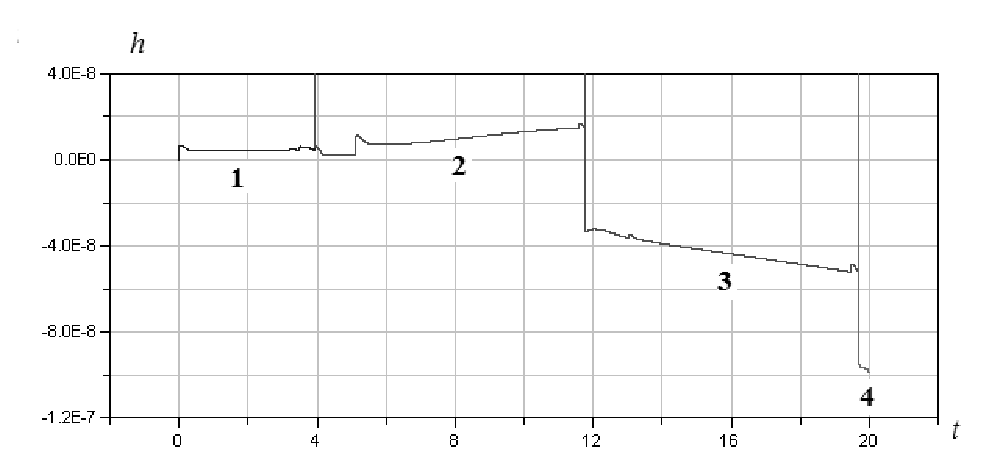
\includegraphics[width=15cm]{content/parts/3_friction/nd/Figure21.eps}}
%\caption{Точность сохранения неудерживающей связи.}
%\label{fig2}
%\end{figure}
%
%\section{Моделирование трения в контакте}

%Конструкция омни-колеса такова, что в каждый данный 
%момент времени имеется имеется только один контакт. Остальные ролики <<висят>>
%над полом. При этом объект механической связи между полом и, <<висящим>> на ободе
%колеса, роликом не исчезает -- алгоритм отслеживания контакта продолжает 
%работать, генерируя в качестве реакций нулевые усилия и моменты.

% Для каждого ролика модели омни-экипажа при контактировании  Это закон Амонтона -- Кулона
% сухого трения. На самом деле вместо этого нами используется кусочно-линейная 
% аппроксимация точного закона трения~\cite{Kosenko2006unilat}. Эта аппроксимация 
% обеспечивает высокую точность вычисления движения тел на больших интервалах 
% времени~\cite{Novozhilov1991}. 

%Для вычисления касательного усилия в точке контакта выбрана модель сухого трения, 
%контакт считается твердотельным. При этом, как известно~\cite{Novozhilov1991}, 
%идеальный <<сухой>> случай реализовать не удается. Вместо разрывной функции 
%sign от скорости относительного скольжения применяется функция линейного насыщения,
%имеющая в окрестности нуля <<крутой>> линейный участок. Для таких функций известен 
%результат~\cite{Novozhilov1991} о близости аппроксимирующего движения и движения, 
%соответствующего <<точному>> случаю разрывной функции sign. 

%В случае фактического выполнения контакта помимо нормальной реакции вычисляется
%также её касательная составляющая, симулирующая силу трения. Для касательного 
%контактного усилия имеется (как и для нормального) множество различных моделей. 
%Мы остановились на реализации простейшего случая -- модели сухого трения при 
%одноточечном твердотельном контакте. При этом, как известно~\cite{Novozhilov1991}, 
%идеальный <<сухой>> случай реализовать не удается. Вместо разрывной функции 
%sign от касательной скорости относительного скольжения контактирующих 
%поверхностей используется её регуляризованный в нуле вариант. В нашем случае 
%вместо функции знака sign применяется функция линейного насыщения, имеющая в 
%окрестности нуля <<крутой>> линейный участок. Для таких функций известен 
%результат~\cite{Novozhilov1991} о близости аппроксимирующего движения и движения, соответствующего <<точному>> случаю разрывной функции sign. Заметим, что и в общем случае реализация модели 
%неудерживающей связи основывается на результатах, обозначенных в 
%работе~\cite{Kosenko2006unilat}.

%\section{Верификация}
В разделе о \textbf{верификации} описана идеализированная безынерционная модель и способ проверки построенной модели с трением в сравнении с безынерционной моделью при стремлении суммарной массы роликов к нулю.

Для верификации использованы результаты работы \cite{Borisov2011} как новейшей (на момент проведения исследования) из неголономных моделей динамики свободной тележки с омниколесами на плоскости \cite{Borisov2011, formalskii, ZobovaTatarinovPMM}. Авторы \cite{Borisov2011} принимают простейшую модель омниколеса как плоского диска, для которого скорость точки контакта с опорной поверхностью направлена вдоль прямой, составляющей некоторый угол $\delta$ с плоскостью колеса.
В настоящей работе данная модель реализована с помощью той же технологии, что и модель с трением, построенная в этой главе, проведены испытания обеих и сравниваются результаты.
Максимальная близость решений построенной модели и верификационной достигается при стремлении массы роликов к нулю.

Значения отношения $\eta$ массы ролика к общей массе колеса принимали в обоих случаях значения от $10^{-6}n^{-1}$ до $10^{-1}n^{-1}$ с шагом $1$ по порядку малости (здесь $n$ - фиксированное количество роликов).
Расчеты приведены для случаев 1 и 2 из главы 2 -- вращения экипажа и его прямолинейного движения.

% \subsection{Гипотеза о близости решений}
%В литературе представлены \cite{Borisov2011, formalskii, ZobovaTatarinovPMM} работы, рассматривающие омниколеса в предположении, что массой и инерцией роликов можно пренебречь, налагающие на систему неголономные связи, ограничивающие направление скорости скольжения в точках контакта колес с поверхностью, на которой стоит экипаж, и не вводящие силу трения в контакте, т.е. считающие скольжение идеальным. Эти идеализированные модели имеют существенно меньше степеней свободы, чем "реальный" омниэкипаж, и легче поддаются аналитическому исследованию.\\
%
%Описанные модели можно использовать для верификации построенной физически-ориентированной модели, рассматривая некоторые элементарные виды движений. Максимальное соответствие построенной модели упомянутым неголономным может быть достигнуто при уменьшении вляиния массы роликов на динамику колеса, а именно, при уменьшении их массы с сохранением общей массы колеса с роликами. На этом предположении и основан наш подход к верификации.\\

%\subsection{Проверочная модель}

%Для верификации использованы результаты работы \cite{Borisov2011} как новейшей из неголономных моделей динамики свободной тележки с омниколесами на плоскости.
%Авторы \cite{Borisov2011} принимают простейшую модель омниколеса как плоского диска, для которого скорость точки контакта с опорной поверхностью направлена вдоль прямой, составляющей некоторый угол $\delta$ с плоскостью колеса.
%Данная модель реализована с помощью той же технологии, что и модель с трением, построенная в этой главе, проведены испытания обеих и сравниваются результаты.

%(см. рис.~\ref{fig:bor_wheel_scheme}).

%Связь, наложенная на колесо в таком случае имеет вид
%$$\vec{v_Q}\cdot\vec{\alpha} = 0,$$
%где $\vec{v_Q}$ - скорость точки контакта, $\vec{\alpha}$ - единичный вектор вдоль оси закрепления роликов.\\
%
%\begin{figure}[ht!]
%    \centering
%    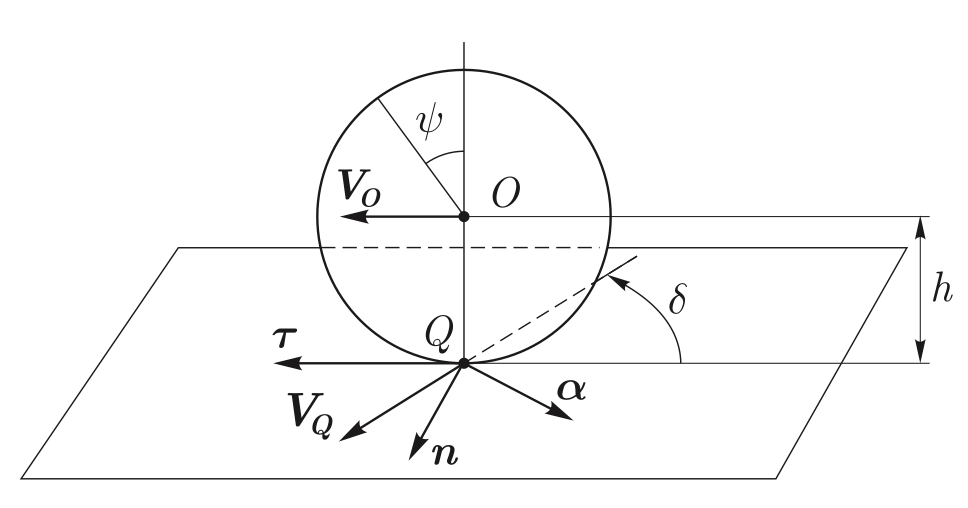
\includegraphics[width=0.75\textwidth]{content/parts/3_friction/diploma/img/art/bor_wheel_scheme.png}
%    \caption{Неголономная модель колеса}
%    \label{fig:bor_wheel_scheme}
%\end{figure}
%
%Авторы \cite{Borisov2011} получают уравнения движения для экипажа с произвольным количеством колес, закрепленных так, что их оси неподвижны относительно платформы, а оси роликов повернуты на произвольные углы относительно плоскостей соответствующих колес (см.рис.~\ref{fig:bor_vehicle}).
%
%\begin{figure}[ht!]
%    \centering
%    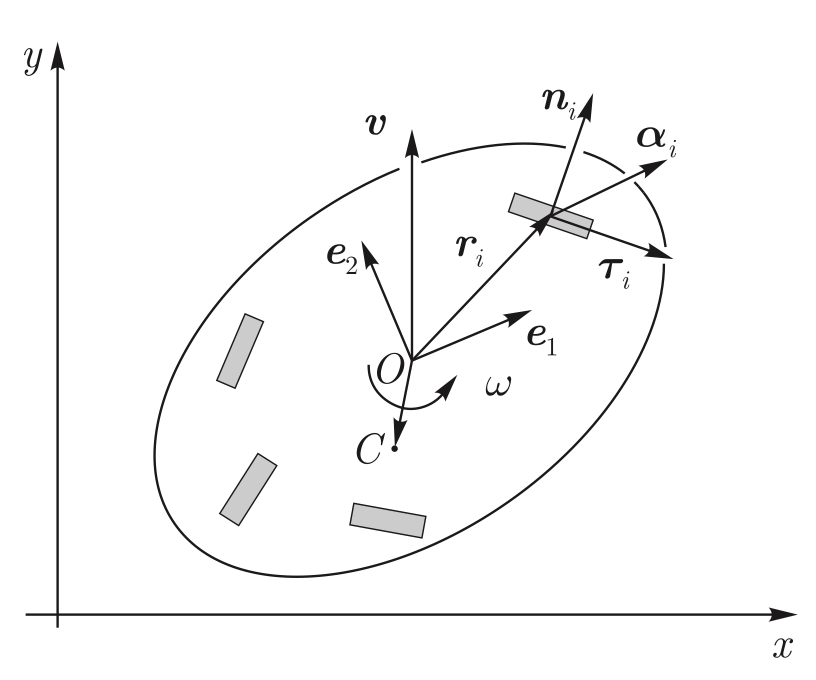
\includegraphics[width=0.75\textwidth]{content/parts/3_friction/diploma/img/art/bor_vehicle.png}
%    \caption{Неголономная модель экипажа}
%    \label{fig:bor_vehicle}
%\end{figure}
%
%Вводится подвижная система отсчета, связанная с платформой экипажа (см.рис.~\ref{fig:bor_vehicle}). Уравнения свободного движения имеют вид:
%\begin{eqnarray*}
%(\Gamma+mE)\dot{\vec{v}} + m\dot{\omega}(J\vec{r_C}+R)+m\omega J(\vec{v} + \omega J\vec{r_C}) = 0,\\
%\hat{I}\dot{\omega} + m(J\vec{r_C}+\vec{r})\cdot\dot{\vec{v}}+m\omega\vec{v}\cdot\vec{r_C} = 0,\\
%\dot{x} = v_1\cos\phi - v_2\sin\phi, \dot{x} = v_1\sin\phi + v_2\cos\phi, \dot{\phi} = \omega,\\
%\Gamma_{kl} = \sum_i \frac{I_i}{s_i^2 h_i^2}\alpha_i^k\alpha_i^l, R = m^{-1}\sum_i \frac{I_i}{s_i^2 h_i^2}(J\vec{r_i}\cdot \alpha_i) \alpha_i,\\
%\hat{I} = I + \sum_i \frac{I_i}{s_i^2 h_i}(J\vec{r_i}\cdot \alpha_i)^2,
%\end{eqnarray*}%
%\newline
%где $\hat{I}$ - суммарный момент инерции системы относительно вертикальной оси, проходящей через начало $O$ подвижной системы отсчета,\newline
%$I$ - момент инерции платформы относительно той же прямой,\newline
%$I_i$ - моменты инерции колес относительно их диаметров,\newline
%$s_i = \sin\delta_i$, $h_i$ - радиусы колес,\newline
%$\vec{r_i}$ - точки закрепления осей колес в подвижной системе,\newline
%$J = \left(\begin{array}{cc}0 & 1\\-1 & 0\end{array}\right)$,\newline
%$x,y,\phi$ - координаты точки $O$ и угол поворота платформы экипажа вокруг вертикальной оси,\newline
%$\vec{v}, \omega$ - вектор скорости точки $O$ и скорость поворота платформы,\newline
%$\vec{r_C}$ - координаты центра масс экипажа в подвижных осях,
%$E$ - единичная матрица.\\

% Данная неголономная модель экипажа также реализована на языке Modelica \cite{ModelicaSpec} как часть упомянутой библиотеки \cite{KosenkoBond}. Таким образом, возможно проведение сравнительного анализа физически-ориентированной и идеализированной моделей и верифкация.


%\subsection{Два типа движений}
%Задавая параметры экипажа, такие как массы его частей, их моменты инерции, геометрические размеры, положения, а также начальные данные - скорость центра масс и угловую скорость платформы, - и выполняя согласованные расчеты для двух реализаций - физической и идеальной - можно получить достаточно близкие движения при достаточно малой доле массы роликов.\\
%
%\begin{figure}[!ht]
%    \centering
%    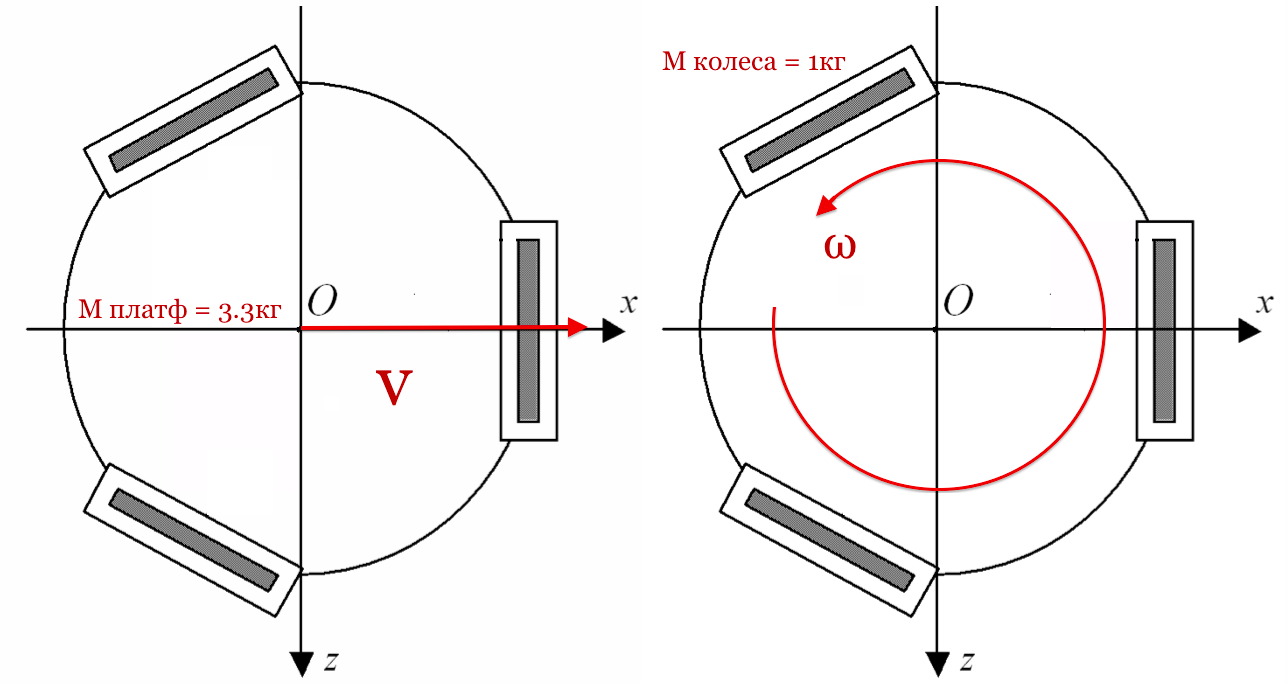
\includegraphics[width=0.95\textwidth]{content/parts/3_friction/diploma/img/art/my_exp_setup.png}
%    \caption{Параметры экспериментов}
%    \label{fig:my_exp_setup}
%\end{figure}

%При выполнении численных экспериментов массы платформы и колес, количество колес, количество роликов, геометрия системы были фиксированы
%(см. рис.~\ref{fig:my_exp_setup})
%. Изменялись начальные данные и доля массы роликов.\\

%Испытания проводились, в частности, и для случая, когда относительная суммарная масса роликов приближается к нулю. В этом случае оказалось, что движение экипажа и омни-колес неограниченно приближаются к соответствующим функциям решения задачи Коши, получаемым в силу дифференциальных уравнений движения, используемых в работе~\cite{Borisov2011}, в которых динамика роликов не учитывается.

%Расчеты приведены для случаев 1 и 2 из главы 2 -- вращения экипажа и его прямолинейного движения.
%Рассмотрены два типа начальных условий $\vec{v}(0) = (v_0, 0, 0)^T, \omega(0) = \omega_0$ (см. рис.~\ref{fig:my_exp_setup}):
%\begin{enumerate}
%\item экипаж имеет начальную линейную скорость в направлении одного из колес и не закручен (ожидаемый результат - центр масс экипажа движется вдоль оси $Ox$, экипаж не вращается),
%\item экипаж закручен вокруг вертикальной оси, проходящей через его центр масс, скорость центра масс равна нулю (ожидаемый результат - экипаж вращается вокруг своей вертикальной оси симметрии, и центр масс покоится).
%\end{enumerate}
%Значения отношения $\eta$ массы ролика к общей массе колеса принимали в обоих случаях значения от $10^{-6}n^{-1}$ до $10^{-1}n^{-1}$ с шагом $1$ по порядку малости (здесь $n$ - фиксированное количество роликов).

%На рис.~\ref{fig:exp_examples} приведены примеры траектории центра масс $y(x)$ и зависимости $\psi(t)$ угла поворота $\psi$ платформы вокруг вертикальной оси, проходящей через её центр, для случаев 1) и 2). Кривые $y(x)$, изображающие траектории центра масс, соответствуют, в сущности, точке - началу координат - в случае $v_0 = 0, \omega_0 = 1$, и отрезку прямой, совпадающей с осью $x$, в случае $v_0 = 1, \omega_0 = 0$, ибо масштаб отображения таков, чтобы были видны отклонения от точных значений, возникающие в силу вычислительной погрешности, но сами эти отклонения имеют порядок малости, позволяющий считать их нулевыми. Аналогичное утверждение верно и для зависимости угла поворота платформы $\psi$ от времени в случае поступательного движения - полученная зависимость близка к постоянной.\\

%Представлены результаты нескольких численных экспериментов.
Во всех случаях величины координат центра масс экипажа на плоскости и угла его поворота относительно вертикальной оси, проходящей через центр масс, совпадают между построенной нами моделью и верификационной идеализацией, с точностью до относительной погрешности величины порядка $10^{-8}$. Также представлена абсолютная величина скорости скольжения в точке контакта в физической модели. Видно, что скольжение имеет место при нахождении точки контакта в окрестности острых концов роликов, причем выражено тем ярче, чем тяжелее ролики.\\

%Ниже представлены результаты нескольких численных экспериментов. Во всех случаях величины, изображенные на рис.~\ref{fig:exp_examples}, демонстрируют поведение, не различимое в масштабе рис.~\ref{fig:exp_examples}, и поэтому приведены лишь расхождения между построенной нами моделью и верификационной идеализацией, которые и представляют интерес. Также представлена абсолютная величина скорости скольжения в точке контакта в физической модели.\\

%Графики зависимости скорости скольжения от времени показывают, что скольжение имеет место в окрестности момента смены роликов. Это объясняется тем, что для идеального качения в эти моменты ролику необходима бесконечная угловая скорость собственного вращения, ибо его размер вблизи вершины стремится к нулю. Видно, что с ростом доли массы роликов в общей массе колеса скольжение в контакте становится существеннее, изменяясь от пренебрежимо малого при $\eta = 10^{-6}$ до весьма существенного уже при $\eta = 10^{-3}$. Тем не менее, расхождения траектории и угла поворота платформы малы, а скольжение наблюдается лишь в точках колеса, которые в промышленных конструкциях не присутствуют (см. Обзор), что и позволяет считать верификацию проведенной.
%\newpage

% EXAMPLES
%\begin{figure}[h]
%\centering
%\begin{subfigure}{.47\textwidth}
%    \centering
%    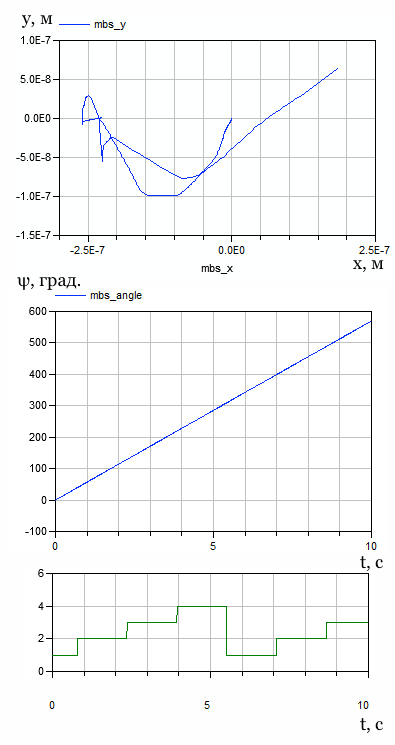
\includegraphics[width=\textwidth]{content/parts/3_friction/diploma/img/res/example_v_0_0_omega_1_frac_1e-1_n_4_time_10s.png}
%    \caption{$\eta = 0,1, v_0 = 0, \omega_0 = 1$}
%    \label{fig:exp_example_omega}
%\end{subfigure}%
%\hspace{5pt}
%\begin{subfigure}{.47\textwidth}
%    \centering
%    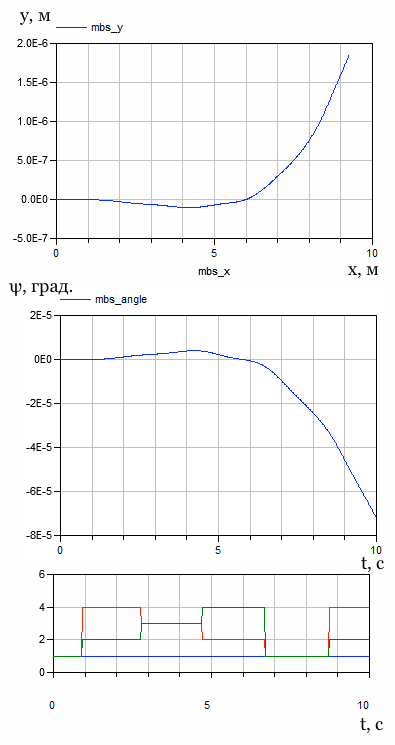
\includegraphics[width=\textwidth]{content/parts/3_friction/diploma/img/res/example_v_1_0_omega_0_frac_1e-1_n_4_time_10s.png}
%    \caption{$\eta = 0,1, v_0 = 1, \omega_0 = 0$}
%    \label{fig:exp_example_v}
%\end{subfigure}
%\caption{Примеры траекторий, характера изменения угла и смены номеров роликов в контакте для двух типов начальных условий. На нижнем графике - номер ролика в контакте, см. рис.~\ref{OmniWheel}}
%\label{fig:exp_examples}
%\end{figure}
%\newpage
%
%\begin{figure}[h]
%\begin{center}\begin{equation*}\begin{array}{cc}
%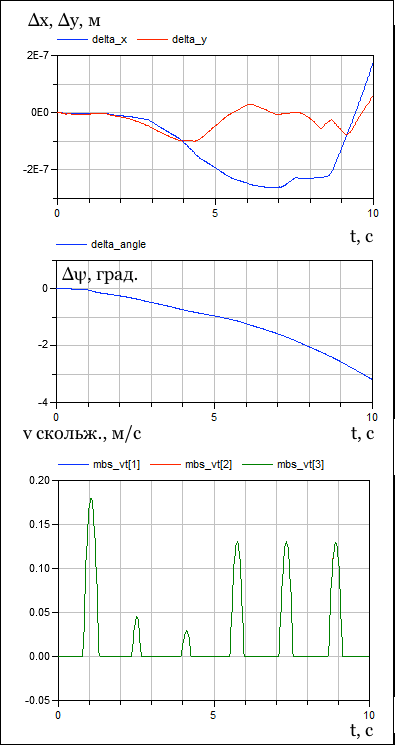
\includegraphics[width=7cm, viewport=0 0 395 745,clip]{content/parts/3_friction/diploma/img/res/comparison_v_0_0_omega_1_frac_1e-1_n_4_time_10s.png} & 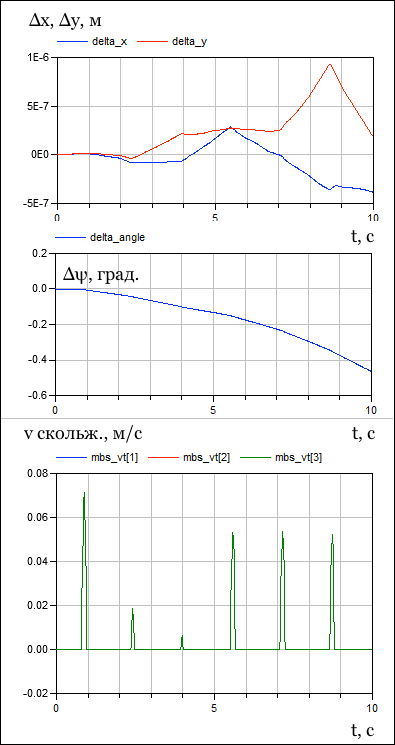
\includegraphics[width=7cm, viewport=0 0 395 745,clip]{content/parts/3_friction/diploma/img/res/comparison_v_0_0_omega_1_frac_1e-2_n_4_time_10s.png}\\
%\eta = 0,1, v_0 = 0, \omega_0 = 1 & \eta = 0,01, v_0 = 0, \omega_0 = 1\\
%\end{array}\end{equation*}\end{center}
%\caption{Вращение экипажа с трением вокруг вертикальной оси}
%\end{figure}
%\newpage
%
%\begin{figure}[h]
%\begin{center}\begin{equation*}\begin{array}{cc}
%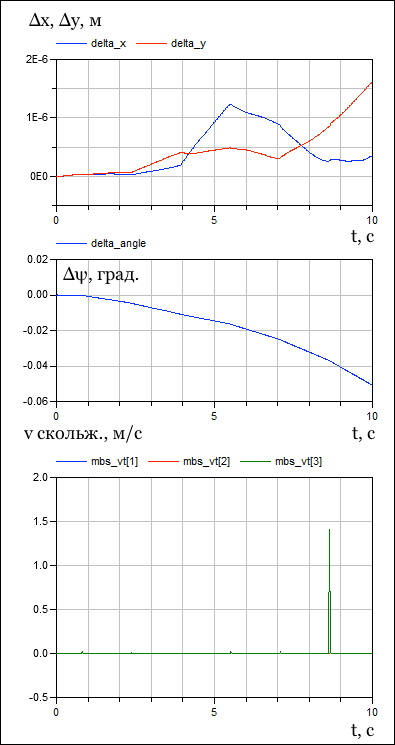
\includegraphics[width=7cm, viewport=0 0 395 745,clip]{content/parts/3_friction/diploma/img/res/comparison_v_0_0_omega_1_frac_1e-3_n_4_time_10s.png} & 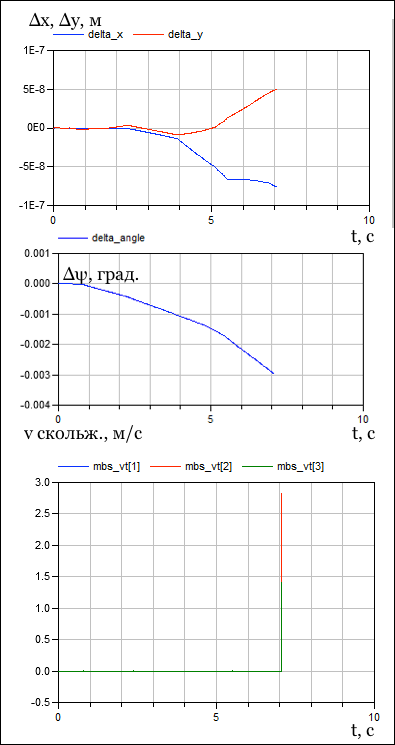
\includegraphics[width=7cm, viewport=0 0 395 745,clip]{content/parts/3_friction/diploma/img/res/comparison_v_0_0_omega_1_frac_1e-4_n_4_time_10s.png}\\
%\eta = 0,001, v_0 = 0, \omega_0 = 1 & \eta = 0,0001, v_0 = 0, \omega_0 = 1\\
%\end{array}\end{equation*}\end{center}
%\caption{Вращение экипажа с трением вокруг вертикальной оси}
%\end{figure}
%\newpage
%
%\begin{figure}[h]
%\begin{center}\begin{equation*}\begin{array}{cc}
%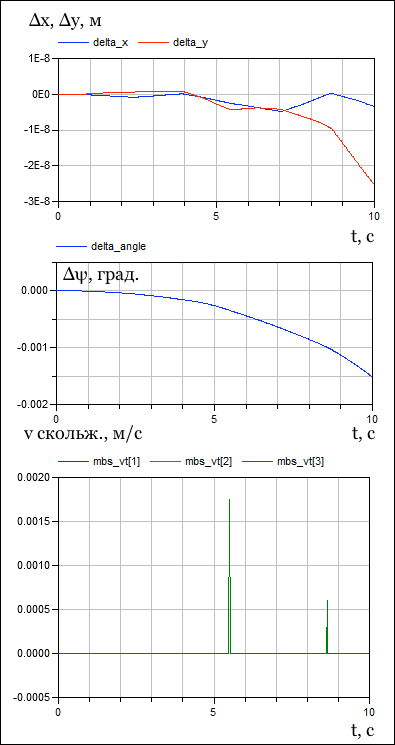
\includegraphics[width=7cm, viewport=0 0 395 745,clip]{content/parts/3_friction/diploma/img/res/comparison_v_0_0_omega_1_frac_1e-5_n_4_time_10s.png} & 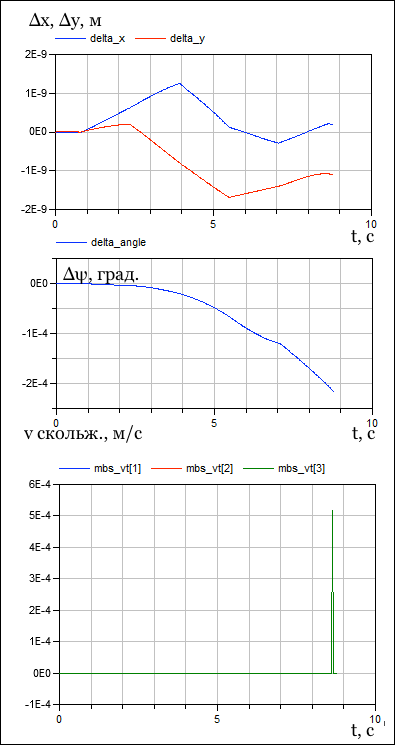
\includegraphics[width=7cm, viewport=0 0 395 745,clip]{content/parts/3_friction/diploma/img/res/comparison_v_0_0_omega_1_frac_1e-6_n_4_time_10s.png}\\
%\eta = 10^{-5}, v_0 = 0, \omega_0 = 1 & \eta = 10^{-6}, v_0 = 0, \omega_0 = 1\\
%\end{array}\end{equation*}\end{center}
%\caption{Вращение экипажа с трением вокруг вертикальной оси}
%\end{figure}
%\newpage
%
%\begin{figure}[h]
%\begin{center}\begin{equation*}\begin{array}{cc}
%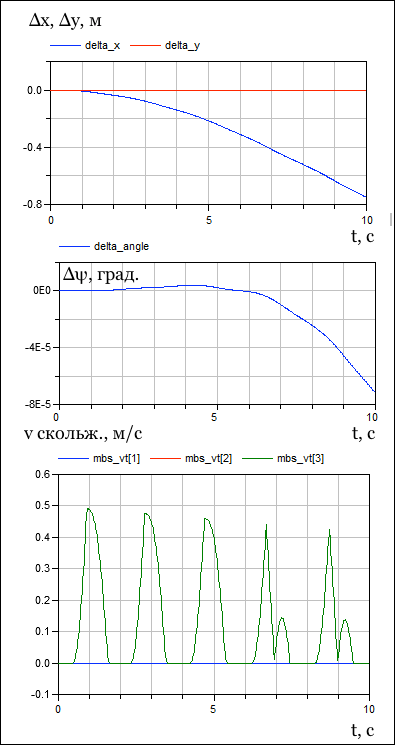
\includegraphics[width=7cm, viewport=0 0 395 745,clip]{content/parts/3_friction/diploma/img/res/comparison_v_1_0_omega_0_frac_1e-1_n_4_time_10s.png} & 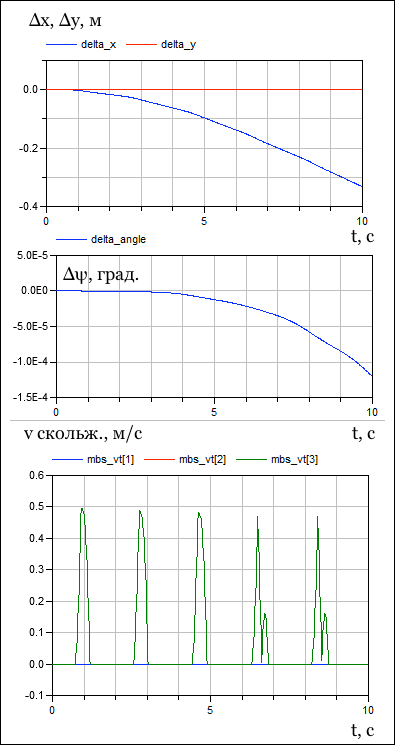
\includegraphics[width=7cm, viewport=0 0 395 745,clip]{content/parts/3_friction/diploma/img/res/comparison_v_1_0_omega_0_frac_1e-2_n_4_time_10s.png}\\
%\eta = 0,1, v_0 = 1, \omega_0 = 0 & \eta = 0,01, v_0 = 1, \omega_0 = 0\\
%\end{array}\end{equation*}\end{center}
%\caption{Вращение экипажа с трением по прямой}
%\end{figure}
%\newpage
%
%\begin{figure}[h]
%\begin{center}\begin{equation*}\begin{array}{cc}
%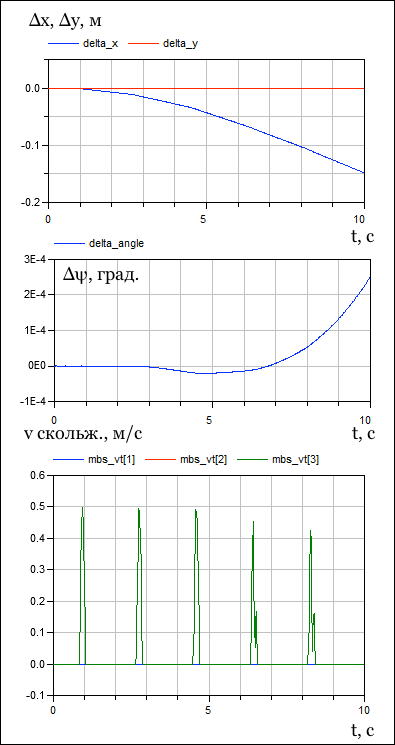
\includegraphics[width=7cm, viewport=0 0 395 745,clip]{content/parts/3_friction/diploma/img/res/comparison_v_1_0_omega_0_frac_1e-3_n_4_time_10s.png} & 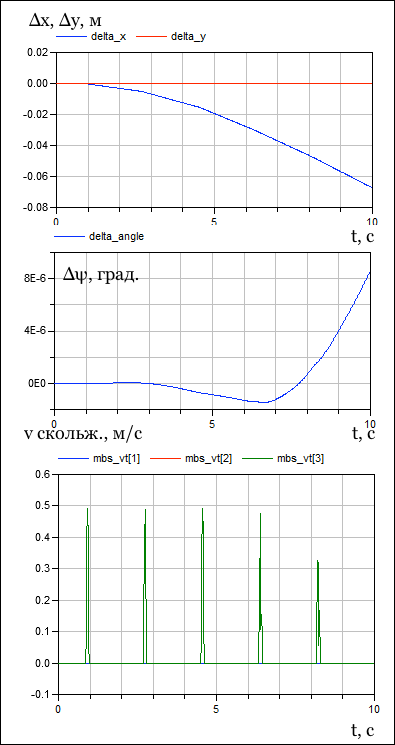
\includegraphics[width=7cm, viewport=0 0 395 745,clip]{content/parts/3_friction/diploma/img/res/comparison_v_1_0_omega_0_frac_1e-4_n_4_time_10s.png}\\
%\eta = 0,001, v_0 = 1, \omega_0 = 0 & \eta = 0,0001, v_0 = 1, \omega_0 = 0\\
%\end{array}\end{equation*}\end{center}
%\caption{Вращение экипажа с трением по прямой}
%\end{figure}
%\newpage
%
%
